\section{Problem 4: communication effectiveness and conservation}\label{sec:q4}

\subsection{Why a product, not a weighted sum}\label{sec:q4-form}

The problem asks for an index that integrates signal fidelity, response-combination
probabilities and context, with an explicit functional form and an ecological interpretation of
its weights. We define the Communication Effectiveness Index as
\begin{equation}\label{eq:cei}
  \boxed{\;\mathrm{CEI}(d \mid c, t) \;=\; F_t(d)\;\times\;P_{\mathrm{recruit}}(d \mid c, t)\;}
\end{equation}
where $F_t(d)$ is the composite fidelity of call type $t$ at distance $d$ from
Section~\ref{sec:q2}, and $P_{\mathrm{recruit}}(d\mid c,t)$ is the probability that a bird
approaches or vocalises, estimated from the playback model of Section~\ref{sec:q3} for context
$c$.

The multiplicative form is a modelling decision with a biological justification. A weighted sum
$w_1F+w_2P$ allows compensation: a signal that cannot be heard at all ($F=0$) but is played in a
context where birds are eager to respond ($P=1$) would score the same as an audible signal in an
indifferent context. Ecologically these are not equivalent, because the second case still
transmits information while the first transmits nothing. Multiplication encodes two necessary
conditions: if the signal is not audible it cannot recruit, and if the bird is not willing it
will not recruit, regardless of audibility. The cost of this choice is that $F$ and $P$ are
positively correlated, so the index should be read as a structural decomposition rather than as
a causal product. The data also show that the two factors are not equally distance-dependent:
fidelity falls steeply beyond 64 m, whereas the recruitment probability declines only weakly
with distance (OR 0.87 per $e$-fold, 95\% CI 0.53--1.44, $p=0.59$). The radius is therefore
driven mainly by the physics of the signal, and the behavioural term acts as a near-constant
scaling of it.

\subsection{Components and the ecological meaning of the weights}\label{sec:q4-weights}

The fidelity term is itself a weighted average of three correlations,
\begin{equation}\label{eq:fid}
  F_t(d) = w_{\mathrm{spec}} r_{\mathrm{spec},t}(d)
         + w_{\mathrm{amp}}  r_{\mathrm{amp},t}(d)
         + w_{\mathrm{env}}  r_{\mathrm{env},t}(d),
  \qquad \sum_m w_m = 1 .
\end{equation}

Each component measures a different kind of redundancy, and the weights are therefore
interpreted as hypotheses about which kind of redundancy carries recognition.

\begin{table}[htbp]
  \centering
  \caption{Components of the index and their ecological interpretation.}\label{tab:q4-weights}
  \small
  \begin{tabular}{llll}
    \toprule
    Component & What it preserves & Ecological reading & Weight \\
    \midrule
    $r_{\mathrm{spec}}$ & time--frequency structure & identity of the caller & 1/3 (0.35 under PCA) \\
    $r_{\mathrm{amp}}$ & spectral envelope & timbre and body size & 1/3 (0.35 under PCA) \\
    $r_{\mathrm{env}}$ & temporal fluctuation & rhythm and pulse pattern & 1/3 (0.30 under PCA) \\
    $P_{\mathrm{recruit}}$ & approach or vocalisation & willingness to join & multiplier, not a weight \\
    \bottomrule
  \end{tabular}
\end{table}

The equal weights are the neutral choice, but they are not innocent: the spectrogram and
amplitude-spectrum correlations are strongly correlated across call types ($r=0.81$--$0.97$), so equal
weighting places two thirds of the weight on what is effectively one dimension. The first
principal component of the three correlations gives normalised weights close to equal (about
0.37, 0.35 and 0.29 in our recomputation), so an equal-weight and a principal-component composite
produce similar fidelity curves. We keep equal weights as the baseline because they require fewer
assumptions, and report the principal-component alternative in the sensitivity analysis. The envelope correlation is the only component that is substantially
independent of the other two, and it is also the component that starts lowest (0.65 at 4 m) and
collapses fastest. It therefore acts as the strictest of the three filters, which is why it
deserves weight even though it is small in magnitude.

Context enters through $P_{\mathrm{recruit}}$, because the playback model already conditions on
context. Multiplying by a separate context factor would count it twice; we do not do so.

\subsection{Effective communication radius}\label{sec:q4-radius}

Two calibration rules are defensible, and we report both.

\begin{itemize}[leftmargin=1.6em,itemsep=3pt]
  \item \textbf{Behaviour-limited (primary).} $\kappa = 0.5\,\mathrm{CEI}(50\,\mathrm{m})$, held
        fixed at its baseline value in every scenario, that is,
        the distance at which communication effectiveness has fallen to half of its value at a
        distance where every call type is still fully audible. This rule adapts to the absolute
        level of the index and is the one we use for management advice.
  \item \textbf{Signal-limited (reference).} $F(d)=\tau$, that is, the distance at which the signal
        itself falls below a recognition threshold. This quantity ignores behaviour and is
        reported only for comparison; it is not the quantity the problem asks for.
\end{itemize}

\begin{table}[htbp]
  \centering
  \caption{Effective radii (m). Behaviour-limited radii use $\kappa=0.5\,\mathrm{CEI}(50\,\mathrm{m})$;
  signal-limited radii use $F(d)=0.5$. Brackets: block-bootstrap 95\% interval.}\label{tab:q4-radius}
  \small
  \begin{tabular}{lrrr}
    \toprule
    Criterion & flat & mod & tv \\
    \midrule
    Behaviour-limited, empirical curve & 136.6 [131.4, 143.0] & 174.8 [167.3, 181.1] & 203.4 [198.2, 209.2] \\
    Behaviour-limited, logistic fit & 135.7 & 175.9 & 157.8 \\
    Absolute $\mathrm{CEI}=0.20$, empirical & 115.7 [112.3, 118.7] & 158.7 [149.5, 167.5] & 215.6 [211.0, 220.6] \\
    Signal-limited $F=0.5$ & 84.7 [83.1, 86.4] & 144.6 [140.6, 148.2] & 169.7 [168.6, 170.9] \\
    \bottomrule
  \end{tabular}
\end{table}

The behaviour-limited radius is larger than the signal-limited one for every call type, which is
expected: a bird can respond to a partially degraded signal, so the behavioural boundary lies
beyond the physical one. The gap is largest for flat calls (137 versus 85 m) and smallest for
two-voice calls (203 versus 170 m).

The model-family comparison matters more than the confidence intervals. For two-voice calls the
empirical curve gives 203 m but a logistic fit gives 158 m, a difference of 45 m that dwarfs the
bootstrap interval of $\pm5$ m. The reason is visible in Figure~\ref{fig:q2-fidelity}: the raw
mean fidelity of the two-voice call is non-monotone (it rises from 8 to 64 m), so a monotone
parametric curve must cut through the plateau and cross the threshold earlier. We therefore quote
the two-voice radius as a \emph{range} of 158--203 m rather than as a point estimate.
Figure~\ref{fig:q4-cei} shows the index itself with bootstrap bands.

\begin{figure}[htbp]
  \centering
  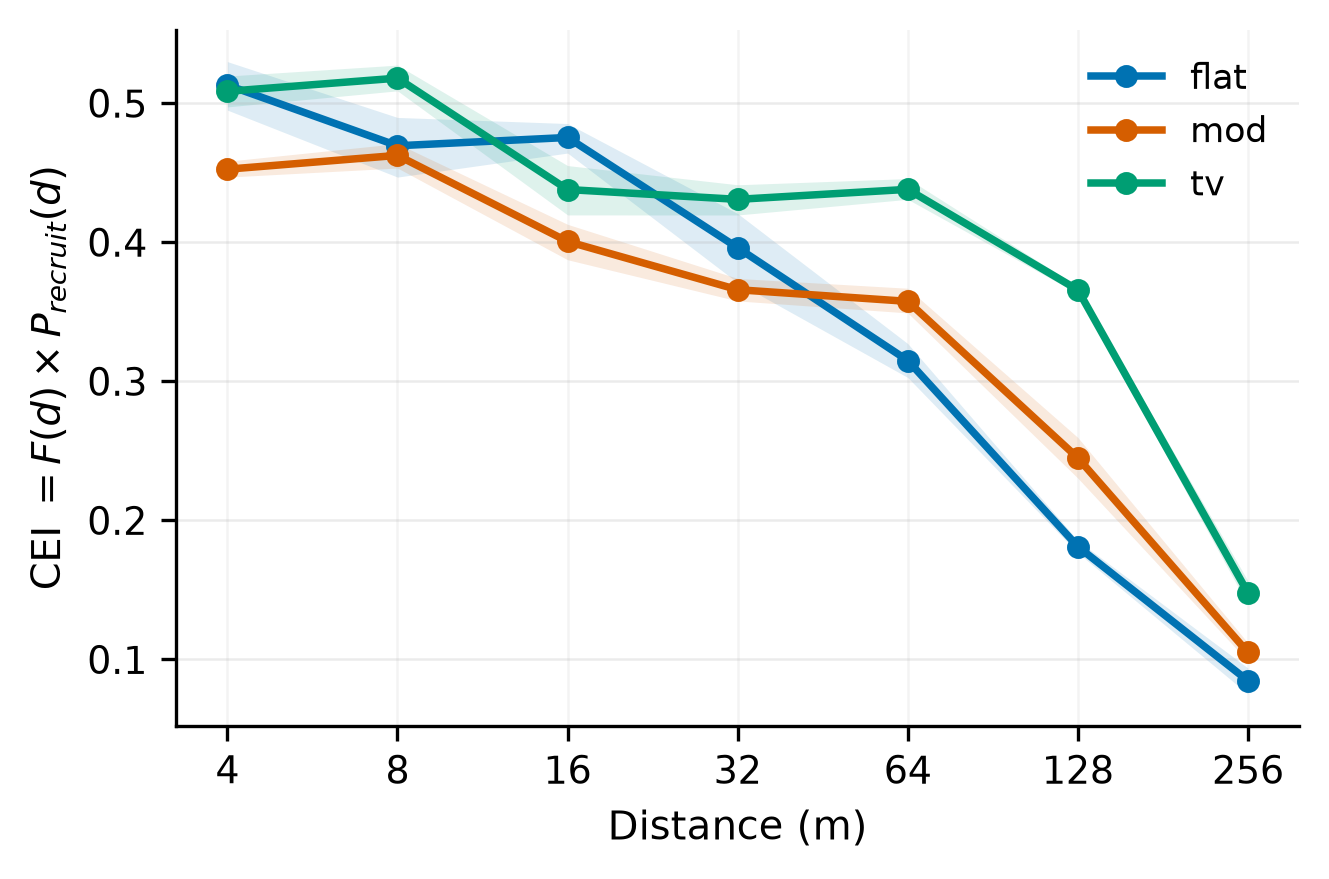
\includegraphics[width=0.42\textwidth]{figs/fig7_cei.png}
  \caption{Communication effectiveness index against distance. The bands reflect fidelity
  sampling only (block bootstrap over the 30 blocks); the recruitment term is held at its point
  estimate. The index is not monotone over 4--64 m because the fidelity curves themselves are
  not.}\label{fig:q4-cei}
\end{figure}

\subsection{Expected number of responders}\label{sec:q4-expected}

The second output the problem permits is the expected number of responding individuals. Let
$p(n)$ be the empirical distribution of group size (139 experiments; median 8, interquartile
range 3--15, mean 10.75, maximum 40). Then
\begin{equation}\label{eq:expected}
  \E[N_{\mathrm{resp}}\mid d] \;=\; \rho \sum_{n} p(n)\; n\; \Prob(\text{any}\mid n,d),
\end{equation}
where $\rho$ is the fraction of individuals in a responding group that actually participate.
The probability in Equation~\eqref{eq:expected} is the probability of \emph{any} response, not
$P_{\mathrm{recruit}}$: the two outputs answer different questions. The index asks how strong the
communication channel is and uses the narrower recruitment event (approach or vocalisation),
whereas the expected-responder count asks how many birds arrive and therefore keeps the broader
any-response event. The
data contain no individual marks, so $\rho$ is not identifiable and is treated as a sensitivity
parameter rather than estimated.

\begin{table}[htbp]
  \centering
  \caption{Expected number of responders by distance and call type, for $\rho=1$ and $\rho=0.5$.}\label{tab:q4-expected}
  \small
  \begin{tabular}{lrrrrrr}
    \toprule
    & \multicolumn{3}{c}{$\rho = 1$} & \multicolumn{3}{c}{$\rho = 0.5$} \\
    \cmidrule(lr){2-4}\cmidrule(lr){5-7}
    Distance (m) & flat & mod & tv & flat & mod & tv \\
    \midrule
    4 & 8.78 & 9.02 & 9.41 & 4.39 & 4.51 & 4.71 \\
    50 & 5.03 & 5.44 & 6.20 & 2.51 & 2.72 & 3.10 \\
    100 & 3.87 & 4.26 & 5.01 & 1.93 & 2.13 & 2.51 \\
    150 & 3.24 & 3.60 & 4.33 & 1.62 & 1.80 & 2.16 \\
    256 & 2.50 & 2.81 & 3.47 & 1.25 & 1.41 & 1.73 \\
    \bottomrule
  \end{tabular}
\end{table}

Because $\rho$ enters linearly it scales every entry of Table~\ref{tab:q4-expected} without
changing the ordering of call types. Sweeping it over the full range requested by the problem,
from 0.1 to 1.0, gives at 100 m the triplets (0.39, 0.43, 0.50) at $\rho=0.1$, (1.93, 2.13, 2.51)
at $\rho=0.5$ and (3.87, 4.26, 5.01) at $\rho=1$. The ratio between call types is invariant by
construction, which is the point: the one parameter we cannot estimate cannot explain away the
difference between the call types.

\subsection{Scenarios and sensitivity}\label{sec:q4-sens}

Table~\ref{tab:q4-scen} and Figure~\ref{fig:q4-scen} report a baseline plus six
perturbations: two thresholds taken from the problem's examples (0.5 to 0.6 and 0.7), two
reductions in all three correlations (5 and 20 percentage points), a 3 dB noise increase, and one
impairment of recruitment (implemented as a deterioration of sea state).

\begin{table}[htbp]
  \centering
  \caption{Behaviour-limited radius (m) under seven scenarios.}\label{tab:q4-scen}
  \small
  \begin{tabular}{lrrr}
    \toprule
    Scenario & flat & mod & tv \\
    \midrule
    Baseline & 136.6 & 174.8 & 203.4 \\
    Recognition threshold 0.6 & 102.4 & 141.1 & 170.8 \\
    Recognition threshold 0.7 & 77.8 & 109.1 & 143.3 \\
    Correlations $-5$ percentage points & 128.3 & 166.8 & 196.2 \\
    Correlations $-20$ percentage points & 107.1 & 140.3 & 171.0 \\
    Noise $+3$ dB (fidelity $-0.10$) & 102.4 & 141.1 & 170.8 \\
    Sea state (recruitment $\times0.8$) & 107.1 & 140.3 & 171.0 \\
    \bottomrule
  \end{tabular}
\end{table}

\begin{figure}[htbp]
  \centering
  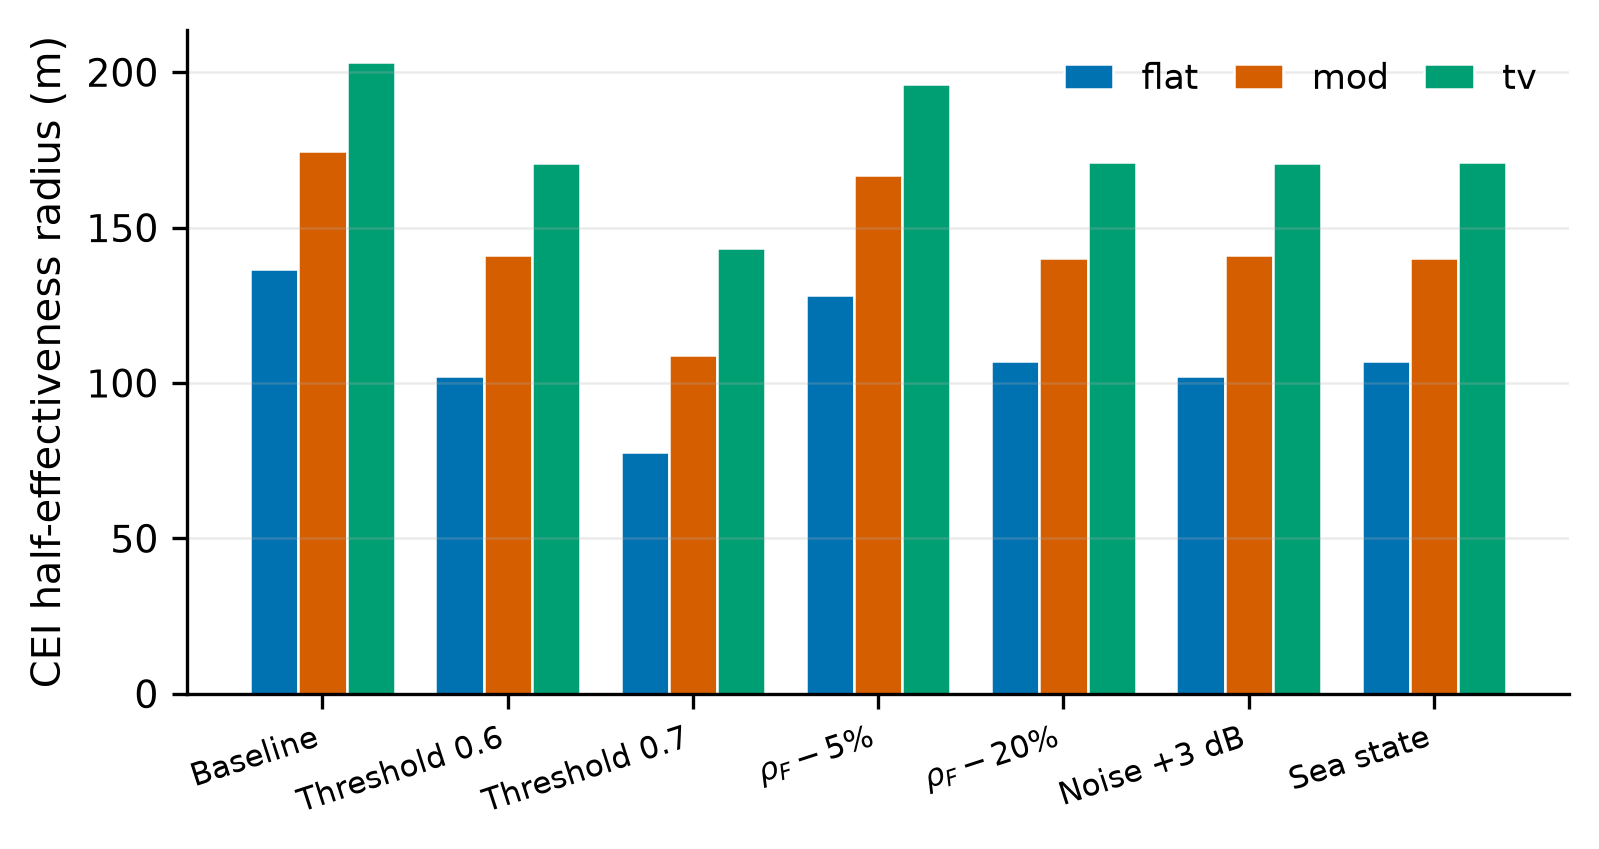
\includegraphics[width=0.52\textwidth]{figs/fig8_scenarios.png}
  \caption{Behaviour-limited radii under the seven scenarios of Table~\ref{tab:q4-scen}.}\label{fig:q4-scen}
\end{figure}

Three results stand out. First, the threshold is the most consequential single choice: moving from
0.5 to 0.7 shortens the two-voice radius from 203 to 143 m, a 30\% reduction. Second, the ranking
of call types is stable across the seven rows --- two-voice remains first and flat last.
The exception to this stability does not appear in the table: it appears in the weight
sensitivity of Section~\ref{sec:q2-sens}, where an envelope-heavy weighting reverses the order.
Third, two pairs of rows are numerically identical by construction. Threshold 0.6 and the 3 dB
noise scenario coincide because both were implemented as a shift of $-0.10$ in fidelity, and the
$-20$ percentage-point correlation reduction coincides with the sea-state scenario because both
were implemented as a multiplication of the index by 0.8. These are limitations of a
one-dimensional scenario design, not coincidences in the data; a finer noise model would require
an explicit signal-to-noise calculation that the supplied data do not support.

The exception is the envelope weight. If the envelope correlation is given weight 0.5 instead of
one third, the two-voice radius at $\tau=0.7$ collapses to 12.1 m while the modulated radius
remains at 66.8 m. The reason is that the two-voice envelope correlation is the lowest of the
three call types at 256 m (0.139), even though its spectrogram correlation is the highest. The
statement ``two-voice calls travel furthest'' is therefore true for the spectral metrics and false
for the envelope metric, and the equal-weight index sits between the two. This is the single
largest structural uncertainty in the analysis, and it is why Section~\ref{sec:discussion}
reports a range rather than a number.

\subsection{Conservation recommendations}\label{sec:q4-rec}

The index translates into four concrete recommendations and one caveat.

\begin{enumerate}[leftmargin=1.8em,itemsep=3pt]
  \item \textbf{A 200 m noise-management buffer around foraging hotspots.} The behaviour-limited
        half-effectiveness radius of the two-voice call is 203 m on the empirical curve and 158 m
        under a logistic fit. A 200 m buffer approximately covers the empirical estimate (203 m); a precautionary
        manager who prefers the conservative estimate would choose 160 m. We recommend 200 m as
        the primary figure and state the 160 m alternative explicitly.
  \item \textbf{A 3 dB limit on vessel noise in the 0.5--2 kHz band.} The first fundamental of
        all three call types lies between 221 and 334 Hz, and the 75th percentile of the spectral
        energy lies near 1.1 kHz, so the 0.5--2 kHz octave band carries most of the signal energy
        as well as most of the engine noise. A 3 dB increase in that band shortens the effective
        radius to 102--171 m (Table~\ref{tab:q4-scen}), if a 3 dB increase were equivalent to the
        assumed 0.10 drop in fidelity used to build that scenario.
  \item \textbf{Seasonal and diurnal timing.} The playback data were collected in a single season
        and do not identify a diel pattern; we therefore recommend that any restriction be
        evaluated against a monitoring series before being made permanent.
  \item \textbf{Monitoring metric.} The spectrogram correlation of two-voice calls at 128 m
        (0.740) is the most sensitive of the available indicators to long-range change, and it is
        the one we recommend for tracking. The envelope correlation should not be used as the
        primary indicator, because it is both the most variable and the least favourable to the
        two-voice call.
\end{enumerate}

The caveat is that all of these numbers come from a single site, a single season and 139 paired
trials. They are precautionary recommendations, not causal guarantees: a buffer derived from
this index is expected to preserve the \emph{opportunity} for acoustic contact, not to guarantee
that recruitment succeeds.
